\documentclass[a4paper]{report}

% Utilisation de tous les packages nécéssaires

\usepackage[utf8]{inputenc}%           gestion des accents (source)
\usepackage[T1]{fontenc}%              gestion des accents (PDF)
\usepackage[british,UKenglish,USenglish,english,american]{babel}%          		 gestion de l'anglais
\usepackage{textcomp}%                 caractères additionnels
\usepackage{lmodern}%                  police de caractère
\usepackage[left=2cm,right=2cm,top=3cm,bottom=3cm]{geometry}%                 gestion des marges
\usepackage{graphicx}%                 gestion des images
\usepackage{ulem}
\graphicspath{{Images/}}
\usepackage{array}%                    gestion améliorée des tableaux
\usepackage{calc}%                     syntaxe naturelle pour les calculs
\usepackage{amsmath}
\usepackage{soul}
\usepackage{fancyhdr}
\usepackage{graphicx}
\usepackage{colortbl}
\usepackage{color}
\usepackage{listings}
\usepackage{url}
\usepackage[colorlinks,linkcolor=black]{hyperref}
\usepackage{amsfonts}
\usepackage{amssymb}
\usepackage{caption}
\usepackage{float}
\usepackage{enumitem}
\usepackage{pstricks,pst-plot,pstricks-add}
\graphicspath{ {graficas/} }
%\captionsetup[figure]{labelformat=empty}
\renewcommand{\lstlistingname}{}
\lstset{
language = {SQL},
frame = single,
basicstyle=\small,
keywordstyle = \bf \color{red},
commentstyle = \color[gray]{0.5},
numbers=left,
numberstyle=\small,
stepnumber=2,
numbersep=7pt,
showstringspaces = false,
tabsize=3,
%keywords = {UNSIGNED, TINYINT, NOT, NULL, MEDIUMINT, "CREATE TABLE", PRIMARY, KEY, YEAR}
}

\setlength{\headheight}{25pt}
\setlength{\parskip}{1ex plus 0.5ex minus 0.2ex}
\setlength{\parindent}{0cm}
\newcommand{\hsp}{\hspace{20pt}}
\newcommand{\HRule}{\rule{\linewidth}{0.5mm}}

\hypersetup{
colorlinks=true, %colorise les liens
breaklinks=true, %permet le retour à la ligne dans les liens trop longs
urlcolor= blue, %couleur des hyperliens
linkcolor= black, %couleur des liens internes
citecolor=blue,    %couleur des liens de citations
}
\title{Neural Networks KU WS18 - Task 2 \\ Classification of a variant of the isolet dataset}
\author{Luis Moran Cordon 11806980 \\ Quentin Loiseau 11805618}



\begin{document}
\maketitle

\pagestyle{fancy}
\fancyhead[R]{}
\fancyhead[L]{
\includegraphics[scale=0.35]{TU_Graz_logo.png}}

\chapter{Purpose of the second task}

\section{First Implementation of a Feedforward Neural Network}
\paragraph{} After discovering a lot of important theorical aspects during the Lecture of Neural Networks and the first Task of the practical, the second task challenged the student to implement a first Feedforward Neural Network.
This works implied to be able to use most of the concepted seen in class. The main requirements were to normalize the sample of data, use the stochastic gradient descent, evaluate the performance of the network, use early stopping. It was also asked to search for the best meta-parameter, as the learning rate or the architecture of the network. Finally, we had to provide all our results in this report - submitted with the code on the teach center.
\paragraph{} To do so, we had to use the library Tensorflow 1.5 in Python 3, and then train this Neural Network to classify data from a variant of the isolet dataset. It was also interesting to try to get the best results possible in term of percentage of misclassified examples.

\section{Data Set}
The data set is derivated from the so called "isolet" dataset - standing for "Isolated Letter Speech Recognition" dataset. To discribe those data, perharps the best way is to quote the creators of the data from the information part :
\\"\textit{150 subjects spoke the name of each letter of the alphabet twice. Hence, we have 52 training examples from each speaker. The speakers are grouped into sets of 30 speakers each, and are referred to as isolet1, isolet2, isolet3, isolet4, and isolet5. The data appears in isolet1+2+3+4. Data in sequential order, first the speakers from isolet1, then isolet2, and so on.  The test set, isolet5, is a separate file.}" 

\chapter{Implementation of the Neural Network}
\section{Organization of the code}
\paragraph{}Our code is organized on a quite common way concerning Feedforward Neural Networks, according to the Tutorial we've had at our disposition. We tried to make it readable, divided in 3 files along with some commentaries to follow its path. The heart of the code (programHL.py) has been done as follows :
\begin{itemize}
\item Load of the data via the function load\_isolet.
\item Normalization of the data via normalizeDataNN.
\item Creation of the architecture of the Neural Network and the variables (especially the trainable ones).
\item Initialization of last features needed before the beginning of the training (cross-entropy, mini-batches...).
\item Training of the Network with a counter dedicated to early stopping.
\item Retraining of the network for the number of epochs that achieved the best validation error.
\end{itemize}
\paragraph{Normalization of the data}
\paragraph{} We have implemented in a special function to do it according to the Min-Max Normalization. This normalization is done according to the following model :
\begin{equation}
X_{normalized} =\frac{X-\min X}{\max X-\min X} - 0.5
\end{equation}
\paragraph{} It results data normalized in the interval [-0.5;0.5]. Another possibility would have been to do it according to the Z-Score Normalization but we didn't knew which one was better to chose in comparison to the other. The Z-Score Normalization takes into account the standard deviation of the data and the result is the following :
\begin{equation}
Y_{normalized} =\frac{Y_{old}- mean}{\sqrt{Var}}
\end{equation}
\paragraph{Definition of the architecture} 
\paragraph{}The moment where we define the architecture of the network before training is crucial. It is one of the main feature we want to optimize in order to obtain the best validation error possible.
\\ In this project we have done a simple architecture of Network, completely feedforward and with some hidden layers.
It might be possible to try different architecture such as RNN or LSTM and get better final results for this task.
\paragraph{} Our code give the possibility to change easily from a Network containing 1 Hidden Layer to 2 or 3. For this, some line in the definition of this architecture are (or aren't) commented. We just have to comment (or uncomment) those before running and choose the number of perceptron in each layer before running in order to get the architecture we want.
\\Between all those models, the only constant concerns the number of inputs and outputs, ruled respectively by the task and the data. There are 300 inputs for the first layer (corresponding to the first 300 features from the original data set), and 26 outputs corresponding to all the letter labels from "a" to "z".
\paragraph{Validation}
\paragraph{}For the validation we produce a random int between 0 and 6228 which is the size of the dataset minus 100 and then we take the 100 first values since that number in the dataset. 
\paragraph{Early Stopping}
\paragraph{}For the training of the validation set we have set an early sopping by saving the best state with a Saver object. If the validation accuracy by at least 0.01 100 times the execution stops. For the training with the test set we have restored the state saved in the validation set training and we also haven´t let the accuracy decrease by 0.01 more than 100 times before stopping the program. We have saved the best state with another Saver. 
\section{Results}
\paragraph{}
We have tried several samples of meta-parameters in our code to get good ideas of what was working (or not) to get good results. Then we have chosen some of the best samples to put them in a table that would give a nice perspective of the results we can have with networks going from 1 to 3 hidden layers. It shows the change of results depending on a change in the architecture of the model, or learning rate.
\\Concerning the activation function we used the ReLU (Rectified Linear Units) as it showed (in average) better results than what we had with tanh or the sigmoïd function. Also we mainly iterated up to 500 steps for the training part.

\paragraph{}Here are the table showing our results concerning the classification of the isolet dataset :

\begin{center}
\begin{tabular}{||c|c|c|c|c||}
\hline
 Learning rate & Hidden layers (units) & Training accuracy & Validation accuracy & Test accuracy  \\ [0.5ex]
\hline
\hline
0.05&1(150)&0.92&0.88&0.748\\
\hline
0.25&1(150)&0.96&1.0&0.752\\
\hline
0.2&1(150)&1.0&0.972&0.76\\
\hline
0.05&1(300)&0.90&0.95&0.754\\
\hline
0.05&1(150) 2(75)&0.90&0.95&0.742\\
\hline
0.05&1(20) 2(20) 3(5)&0.624&0.62&0.634\\
\hline
0.05&1(20) 2 (20)&0.77&0.76&0.692\\
\hline
\end{tabular}
\end{center}

\paragraph{} We can see that the influence of the learning rate is not that determinent in the final results providing that it is not too low or too high. It would be then difficult either to access to a local minima (too low), either to reach this zone because the "jump" is too big (too high).
\\On another perspective, we can see in the last part of the table that the architecture play a really important role concerning the final accuracy. Our results tell us that the best performance are reached in the neural networks made of only one hidden layer, and that the testing accuracy tends to drop if there are too few neurons inside the hidden layers. In the best cases, the final test accuracy was always (at maximum) near the 75% of success (and 25% of miss-classification).

\paragraph{Graphs}
To finish this exercise we present the graphs associated to the results of some example given in the table. The first one shows the cross-entropy over each iteration, and the second one the accuracy over each iteration, sometimes for the training and validation and some times for the testing part.

\begin{figure}[h]
\begin{center}
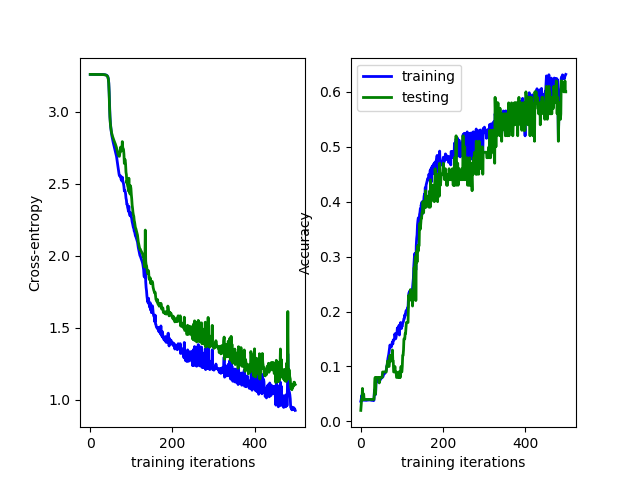
\includegraphics[scale=0.5]{test-20-20-5-0,05.png}
\end{center}
\caption{1(20)2(20)3(5) Validation and training results}
\end{figure}
\begin{figure}[h]
\begin{center}
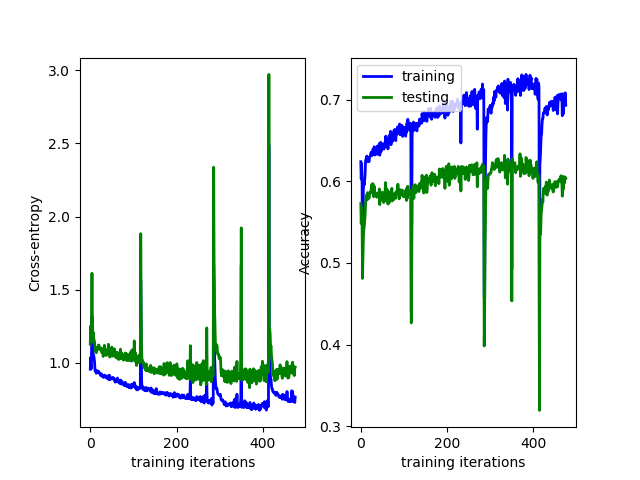
\includegraphics[scale=0.5]{testDeverdadlootroesval202050,05.png}
\end{center}
\caption{1(20)2(20)3(5) Test set results}
\end{figure}
\begin{figure}[h]
\begin{center}
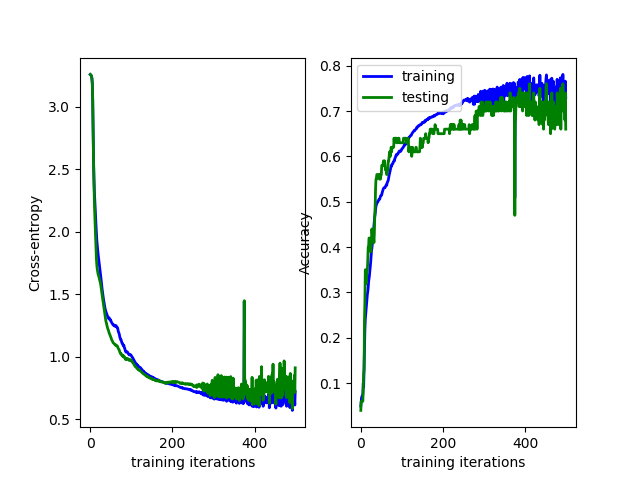
\includegraphics[scale=0.5]{20200,05val.png}
\end{center}
\caption{1(20)2(20) Validation results}
\end{figure}
\begin{figure}[h]
\begin{center}
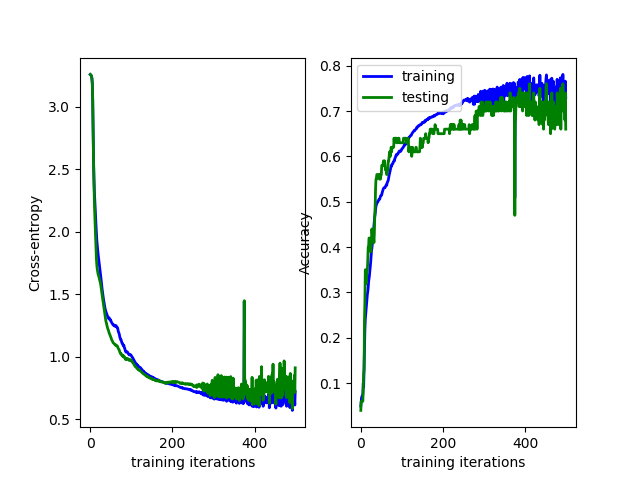
\includegraphics[scale=0.5]{20200,05val.png}
\end{center}
\caption{1(20)2(20) test results}
\end{figure}
\begin{figure}[h]
\begin{center}
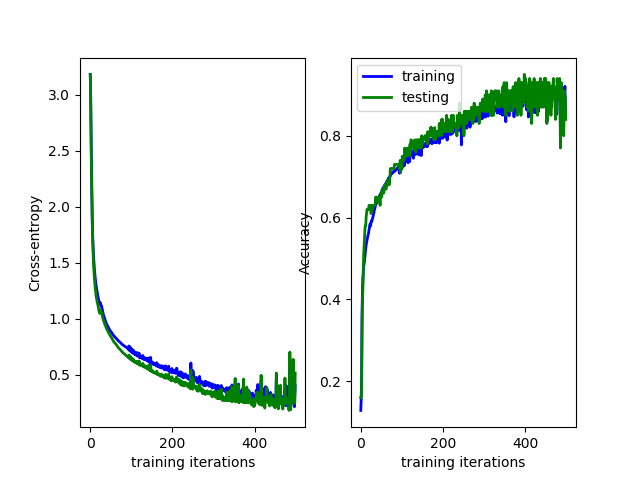
\includegraphics[scale=0.5]{15075val.png}
\end{center}
\caption{1(150)2(75) validation results}
\end{figure}
\begin{figure}[h]
\begin{center}
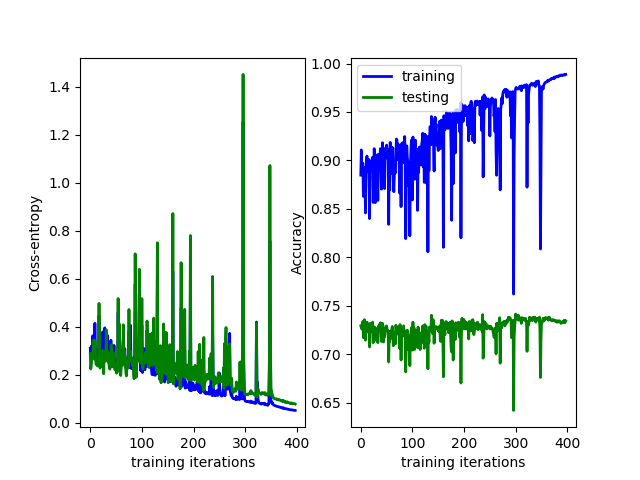
\includegraphics[scale=0.5]{15075test.png}
\end{center}
\caption{1(150)2(75) test results}
\end{figure}
\begin{figure}[h]
\begin{center}
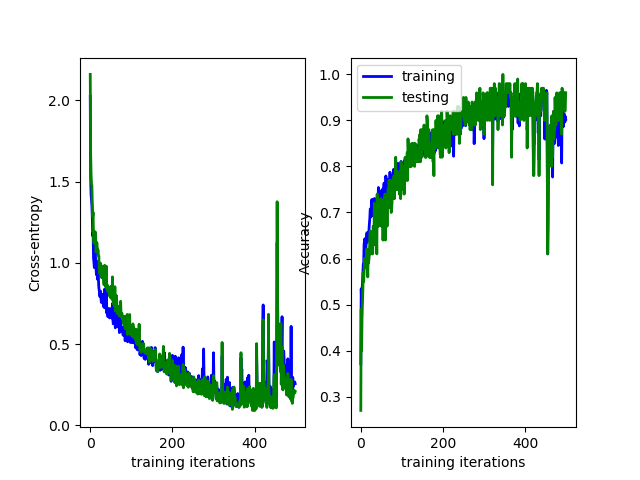
\includegraphics[scale=0.5]{150025.png}
\end{center}
\caption{1(150) 0.25 learning rate validation results}
\end{figure}
\begin{figure}[h]
\begin{center}
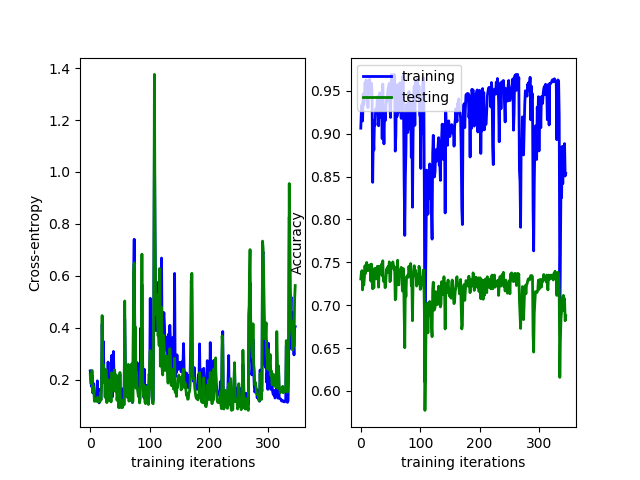
\includegraphics[scale=0.5]{150025test.png}
\end{center}
\caption{1(150) 0.25 learning rate test results}
\end{figure}



\end{document}